\documentclass[12pt,a4paper]{extarticle}
\usepackage{pdfpages}
\usepackage[utf8]{inputenc}
\usepackage{multicol,multirow}
 \usepackage{charter}
\usepackage[
a4paper,
twoside,
bindingoffset=0.5cm,
inner=2cm,
outer=2cm,
top=3cm,
bottom=3cm,
headsep=1.2cm
]{geometry}
\usepackage[sort,numbers]{natbib}
\usepackage{bibentry}
% \usepackage{nyul_thesis}
\usepackage{graphicx}
\usepackage{caption}
\usepackage{setspace}
\usepackage{hyperref}
\usepackage{enumitem}
\usepackage{float}
%\usepackage[euler]{textgreek}

\pagestyle{plain}

\captionsetup[figure]{labelfont={bf},textfont={it}}
\captionsetup[table]{labelfont={bf},textfont={it}}

\begin{document}

\nobibliography*


 \thispagestyle{empty}

 \begin{center}

 \vspace*{2em}

 \large \textbf{Theses of the PhD thesis}
 \vspace*{4em}

 \LARGE \textbf{Title}
 
 \vspace*{4em}
  
 \Large \textbf{FIRSTNAME LASTNAME}

 \vspace*{4em}


% INFO: title can be: assistant professor, associate professor, college professor, professor, professor emeritus
 {\large Supervisor: \\ \textbf{FIRSTNAME LASTNAME, PhD, TITLE} }
 
% INFO: If your have more than one supervisor:
%   {\large Supervisors: \\ \textbf{FIRSTNAME LASTNAME, PhD, TITLE} \\ \textbf{Firstname Lastname, PhD, title}}

 
 \vspace*{4em}
 \large \textbf{ Doctoral School of Computer Science\\University of Szeged}
 
  \vspace*{1em}
 
 \large \textbf{ Department of YOURDEPARTMENT} 

 \vfill

 \large \textbf{YEAR}

 \end{center}
 

 
\newpage
\thispagestyle{empty}
\mbox{}

\newpage

\setcounter{page}{1}
 
\newpage
\section{Introduction}

Brief introduction to the topic. 

Problem statement and motivation.

The PhD thesis presents ... .

The dissertation consists of N major parts. The first chapter presents ..., the N. chapter presents ... .

% INFO: The number of thesis groups can vary based on the major parts of the dissertation.
\section{Title of first thesis group}

Brief introduction to the thesis group.

Problem statement, challenges and motivation.

In Chapter X. of the PhD thesis, a(n) ... is presented.

% INFO: The number of subsections can vary based on how many parts of that particular thesis group has. The details and results have to be brief and straightforward. Use only as much information as the reader needs to understand the problem and the significance of the results.
\subsection{Subsection of the thesis group}

%  If a figure is needed:
% \begin{figure}[b]
%     \centering
%     \includegraphics[width=4in]{Figures/figure_name.png}
%     \caption{Figure caption}
%     \label{figure_label}
% \end{figure}

Brief introduction to the topic 1-2 sentence.

Details of the work.

Main results and significance of the work.

\subsection{Subsection of the thesis group}

%  If a figure is needed:
% \begin{figure}[b]
%     \centering
%     \includegraphics[width=4in]{Figures/figure_name.png}
%     \caption{Figure caption}
%     \label{figure_label}
% \end{figure}

Brief introduction to the topic 1-2 sentence.

Details of the work.

Main results and significance of the work.

\subsection{Subsection of the thesis group}

%  If a figure is needed:
% \begin{figure}[b]
%     \centering
%     \includegraphics[width=4in]{Figures/figure_name.png}
%     \caption{Figure caption}
%     \label{figure_label}
% \end{figure}

Brief introduction to the topic 1-2 sentence.

Details of the work.

Main results and significance of the work.

\section{Title of the second thesis group}

Brief introduction to the thesis group.

Problem statement, challenges and motivation.

In Chapter X. of the PhD thesis, a(n) ... is presented.

\subsection{Subsection of the thesis group}

%  If a figure is needed:
% \begin{figure}[b]
%     \centering
%     \includegraphics[width=4in]{Figures/figure_name.png}
%     \caption{Figure caption}
%     \label{figure_label}
% \end{figure}

Brief introduction to the topic 1-2 sentence.

Details of the work.

Main results and significance of the work.

\subsection{Subsection of the thesis group}

%  If a figure is needed:
% \begin{figure}[b]
%     \centering
%     \includegraphics[width=4in]{Figures/figure_name.png}
%     \caption{Figure caption}
%     \label{figure_label}
% \end{figure}

Brief introduction to the topic 1-2 sentence.

Details of the work.

Main results and significance of the work.

\subsection{Subsection of the thesis group}

%  If a figure is needed:
% \begin{figure}[b]
%     \centering
%     \includegraphics[width=4in]{Figures/figure_name.png}
%     \caption{Figure caption}
%     \label{figure_label}
% \end{figure}

Brief introduction to the topic 1-2 sentence.

Details of the work.

Main results and significance of the work.

\section{Title of the third thesis group}

Brief introduction to the thesis group.

Problem statement, challenges and motivation.

In Chapter X. of the PhD thesis, a(n) ... is presented.

\subsection{Subsection of the thesis group}

%  If a figure is needed:
% \begin{figure}[b]
%     \centering
%     \includegraphics[width=4in]{Figures/figure_name.png}
%     \caption{Figure caption}
%     \label{figure_label}
% \end{figure}

Brief introduction to the topic 1-2 sentence.

Details of the work.

Main results and significance of the work.

\subsection{Subsection of the thesis group}

%  If a figure is needed:
% \begin{figure}[b]
%     \centering
%     \includegraphics[width=4in]{Figures/figure_name.png}
%     \caption{Figure caption}
%     \label{figure_label}
% \end{figure}

Brief introduction to the topic 1-2 sentence.

Details of the work.

Main results and significance of the work.

\subsection{Subsection of the thesis group}

%  If a figure is needed:
% \begin{figure}[b]
%     \centering
%     \includegraphics[width=4in]{Figures/figure_name.png}
%     \caption{Figure caption}
%     \label{figure_label}
% \end{figure}

Brief introduction to the topic 1-2 sentence.

Details of the work.

Main results and significance of the work.

\vspace*{1em}

\section{Contributions of the thesis}
%INFO: The space between the thesis group contributions can be changed using the argument of the \vspace command. In this way the placement can be altered to fit a thesis group full page. In some cases the \newpage command can be used to force the thesis group to a new page.

\vspace*{1em}

In the \textbf {first thesis group}, my contributions are related to ... . Detailed discussion can be found in Chapter X.
\vspace*{1em}
\begin{enumerate}[wide = 0pt, widest = {I/4.}, leftmargin =*]
    \item [I / 1.] I gave a(n) ... . I developed a(n) .... . 
    I showed that .. .
    
    \item [I / 2.] I proposed a(n) ...., and showed ... .
    
    \item [I / 3.] I designed a(n) ...., and proved ... .

\end{enumerate}

\vspace*{1em}
\noindent

In the \textbf {second thesis group}, my contributions are related to ... . Detailed discussion can be found in Chapter X.
\vspace*{1em}
\begin{enumerate}[wide = 0pt, widest = {II/5.}, leftmargin =*]
    \item [II / 1.] I gave a(n) ... . I developed a(n) .... . 
    I showed that .. .
    
    \item [II / 2.] I proposed a(n) ...., and showed ... .
    
    \item [II / 3.] I designed a(n) ...., and proved ... .
\end{enumerate}

\vspace*{1em}
\noindent

In the \textbf {third thesis group}, my contributions are related to ... . Detailed discussion can be found in Chapter X.

\begin{enumerate}[wide = 0pt, widest = {III/5.}, leftmargin =*]
    \item [III / 1.] I gave a(n) ... . I developed a(n) .... . 
    I showed that .. .
    
    \item [III / 2.] I proposed a(n) ...., and showed ... .
    
    \item [III / 3.] I designed a(n) ...., and proved ... .
\end{enumerate}

\vspace*{1em}
\noindent
Table~\ref{tab:summary_table} summarizes the relation between the thesis points and the corresponding publications.
\vspace*{2em}

% INFO: https://www.tablesgenerator.com/latex_tables Use this online tool for the table generation
\begin{table}[h!]
\centering
\caption{Correspondence between the thesis points and my publications.}
\label{tab:summary_table}
\begin{tabular}{|c|c|c|c|c|c|c|c|c|c|c|}
\hline
\multirow{2}{*}{\textbf{Publication}} & \multicolumn{9}{c|}{\textbf{Thesis point}}                                                                                                                                                                                                                                        \\
                                      & \multicolumn{1}{c|}{I/1}       & \multicolumn{1}{c|}{I/2}       & \multicolumn{1}{c|}{I/3}       & \multicolumn{1}{c|}{II/1}      & \multicolumn{1}{c|}{II/2}      & \multicolumn{1}{c|}{II/3}      & \multicolumn{1}{c|}{III/1}     & \multicolumn{1}{c|}{III/2}     & III/3     \\ \hline
{[}1{]}                               & \multicolumn{1}{c|}{}          & \multicolumn{1}{c|}{}          & \multicolumn{1}{c|}{}          & \multicolumn{1}{c|}{}          & \multicolumn{1}{c|}{}          & \multicolumn{1}{c|}{}          & \multicolumn{1}{c|}{}          & \multicolumn{1}{c|}{$\bullet$} &           \\ \hline
{[}2{]}                               & \multicolumn{1}{c|}{$\bullet$} & \multicolumn{1}{c|}{}          & \multicolumn{1}{c|}{}          & \multicolumn{1}{c|}{}          & \multicolumn{1}{c|}{$\bullet$} & \multicolumn{1}{c|}{$\bullet$} & \multicolumn{1}{c|}{}          & \multicolumn{1}{c|}{}          &           \\ \hline
{[}3{]}                               & \multicolumn{1}{c|}{}          & \multicolumn{1}{c|}{}          & \multicolumn{1}{c|}{}          & \multicolumn{1}{c|}{}          & \multicolumn{1}{c|}{}          & \multicolumn{1}{c|}{}          & \multicolumn{1}{c|}{}          & \multicolumn{1}{c|}{}          &           \\ \hline
{[}4{]}                               & \multicolumn{1}{c|}{$\bullet$} & \multicolumn{1}{c|}{}          & \multicolumn{1}{c|}{}          & \multicolumn{1}{c|}{}          & \multicolumn{1}{c|}{$\bullet$} & \multicolumn{1}{c|}{$\bullet$} & \multicolumn{1}{c|}{}          & \multicolumn{1}{c|}{}          &           \\ \hline
{[}5{]}                               & \multicolumn{1}{c|}{}          & \multicolumn{1}{c|}{}          & \multicolumn{1}{c|}{}          & \multicolumn{1}{c|}{}          & \multicolumn{1}{c|}{}          & \multicolumn{1}{c|}{}          & \multicolumn{1}{c|}{$\bullet$} & \multicolumn{1}{c|}{}          &           \\ \hline
{[}6{]}                               & \multicolumn{1}{c|}{}          & \multicolumn{1}{c|}{}          & \multicolumn{1}{c|}{$\bullet$} & \multicolumn{1}{c|}{$\bullet$} & \multicolumn{1}{c|}{}          & \multicolumn{1}{c|}{}          & \multicolumn{1}{c|}{}          & \multicolumn{1}{c|}{}          &           \\ \hline
{[}7{]}                               & \multicolumn{1}{c|}{}          & \multicolumn{1}{c|}{}          & \multicolumn{1}{c|}{}          & \multicolumn{1}{c|}{}          & \multicolumn{1}{c|}{}          & \multicolumn{1}{c|}{}          & \multicolumn{1}{c|}{}          & \multicolumn{1}{c|}{}          & $\bullet$ \\ \hline
{[}8{]}                               & \multicolumn{1}{c|}{}          & \multicolumn{1}{c|}{}          & \multicolumn{1}{c|}{}          & \multicolumn{1}{c|}{}          & \multicolumn{1}{c|}{}          & \multicolumn{1}{c|}{}          & \multicolumn{1}{c|}{}          & \multicolumn{1}{c|}{$\bullet$} &           \\ \hline
{[}9{]}                               & \multicolumn{1}{c|}{}          & \multicolumn{1}{c|}{$\bullet$} & \multicolumn{1}{c|}{}          & \multicolumn{1}{c|}{}          & \multicolumn{1}{c|}{}          & \multicolumn{1}{c|}{}          & \multicolumn{1}{c|}{}          & \multicolumn{1}{c|}{}          &           \\ \hline
\end{tabular}
\end{table}

% INFO: Get the publication list to a new page. If there is too much empty space left on the page before, then comment it out
\newpage
\section*{The author’s publications on the subjects of the thesis}

\vspace*{1em}

\subsection*{Journal publications}

\vspace*{1em}

%INFO: Each enumeration can be in ascending publication year order, oldest publication first, newest publication last
\begin{enumerate}[wide = 0pt, widest = {[4]}, leftmargin =*]

\item[{[1]}] E. Xample, E. Xample2, \textbf{A. Uthor} and E. Xample3
\newblock {A very good title for a journal publication}.
\newblock \emph{Journal name}, Volume, page-page, year.

\vspace*{1em}

\item[{[2]}] \textbf{A. Uthor}, E. Xample, E. Xample2
\newblock {Another very good title for a journal article}.
\newblock \emph{Journal name}, Volume(Issue), page-page, year.

\end{enumerate}

\vspace*{1em}

\subsection*{Full papers in conference proceedings}
\vspace*{1em}

\begin{enumerate}[wide = 0pt, widest = {[4]}, leftmargin =*]

\item[{[3]}] \textbf{A. Uthor} and E. Xample.
\newblock {Conference publication title}.
\newblock In \emph{Proceedings of the Xnd Some Conference}, publisher, page-page, year.
\vspace*{1em}
\item[{[4]}] \textbf{A. Uthor} and E. Xample.
\newblock {Conference publication title}.
\newblock In \emph{Proceedings of the Xnd Some Conference}, publisher, page-page, year.
\vspace*{1em}
\item[{[5]}] \textbf{A. Uthor} and E. Xample.
\newblock {Conference publication title}.
\newblock In \emph{Proceedings of the Xnd Some Conference}, publisher, page-page, year.
\vspace*{1em}
\item[{[6]}] \textbf{A. Uthor} and E. Xample.
\newblock {Conference publication title}.
\newblock In \emph{Proceedings of the Xnd Some Conference}, publisher, page-page, year.
\vspace*{1em}
\item[{[7]}] \textbf{A. Uthor} and E. Xample.
\newblock {Conference publication title}.
\newblock In \emph{Proceedings of the Xnd Some Conference}, publisher, page-page, year.
\vspace*{1em}
\item[{[8]}] \textbf{A. Uthor} and E. Xample.
\newblock {Conference publication title}.
\newblock In \emph{Proceedings of the Xnd Some Conference}, publisher, page-page, year.
\vspace*{1em}
\item[{[9]}] \textbf{A. Uthor} and E. Xample.
\newblock {Conference publication title}.
\newblock In \emph{Proceedings of the Xnd Some Conference}, publisher, page-page, year.
\end{enumerate}

\vspace*{2.00em}

\subsection*{Further related publications}
\vspace*{1em}

\begin{enumerate}[wide = 0pt, widest = {[15]}, leftmargin =*]

\item[{[10]}] \textbf{A. Uthor}, E. Xample, E. Xample2, E. Xample3, E. Xample4, E. Xample5, E. Xample6.
\newblock {Title}.
\newblock In \emph{The Xth International Workshop on Something}, publisher, page-page, year.

\end{enumerate}

\newpage

%INFO Summary on other language, in case it is Hungarian, maximum 1 page, 2000-3000 characters.
\section{Összefoglalás}

Az értekezés ... ismertet, magába foglalva ... . A bemutatott megközelítések közös vonása a ... .

A munka N fő témakörből áll. Az első fejezetben a(z) ... , a második fejezetben a(z) ... , míg a N. fejezetben a(z) ... olvasható.

A fejezetcíme című fejezetben ... . Módszer leírása, eredmény összefoglalása, jelentőség.

A fejezetcíme című fejezetben ... . Módszer leírása, eredmény összefoglalása, jelentőség.

A fejezetcíme című fejezetben ... . Módszer leírása, eredmény összefoglalása, jelentőség.

% Ha kilóg a magyar szöveg akkor fel\-le\-het\-bon\-ta\-ni ilyen módon, ekkor a fordító tudja, hogy hol lehet elválasztani a szót a nyelv helyesírási szabályainak megfelelően.

\newpage

%INFO include the declaration document on only one language (the example includes a hungarian and an english example. It is has to be signed by your supervisor. After all of the co-authors declared that you are the responsible for the results in those thesis points and articles the head of the doctoral school can sign it too. With all of the signs it can be included at the end of the thesis booklet.
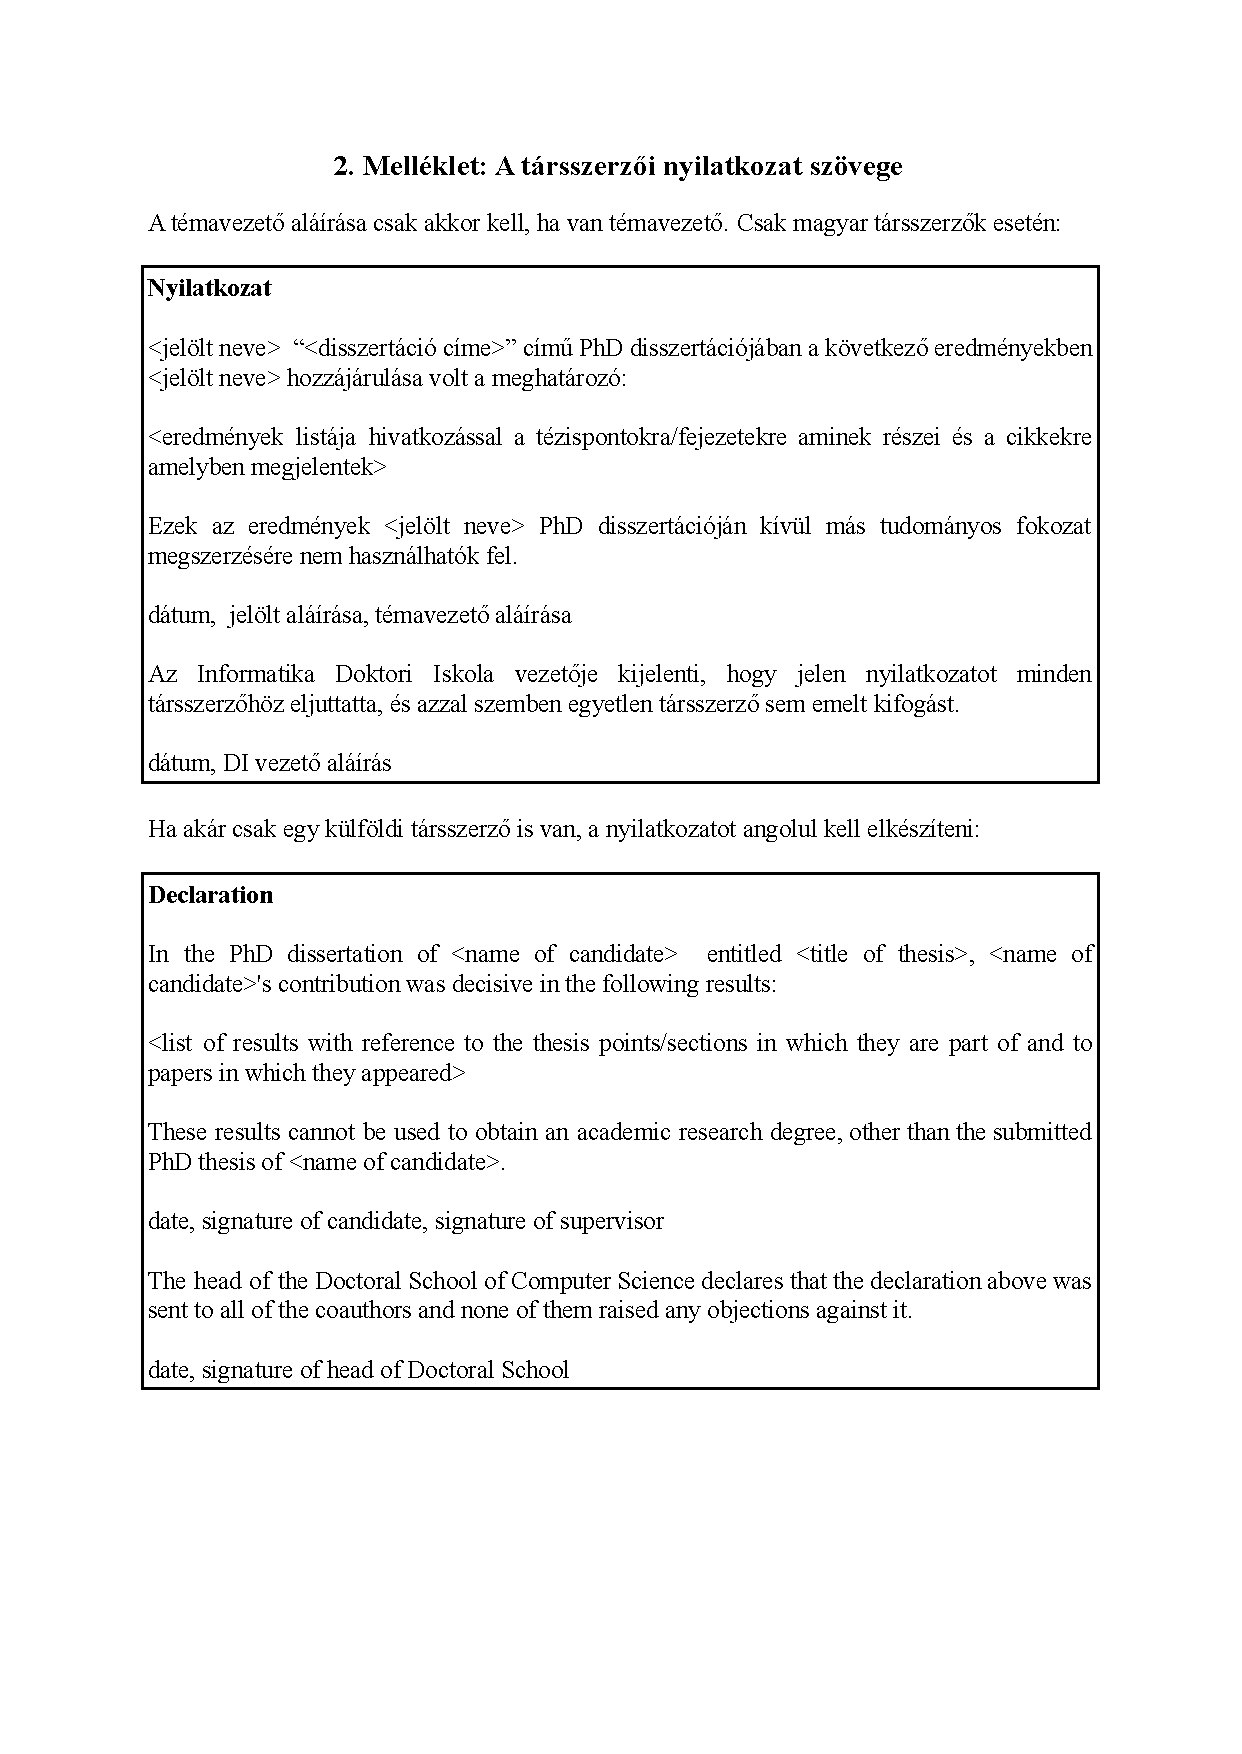
\includepdf[pages=-]{declaration_example.pdf}

\newpage
\thispagestyle{empty}
\mbox{}
\newpage



\end{document}

